% Nome do capítulo
\chapter{Introdução}
% Label para referenciar
\label{cap:1}

% Diminuir espaçamento entre título e texto
\vspace{-1.9cm}

Atualmente há um expressivo crescimento no volume de conteúdo visual, como imagens e vídeos, disponíveis para utilização. Podemos vincular este fato à popularização das tecnologias produtoras destes tipos de conteúdo, como celulares com câmeras, bem como a expansão da Internet e seus canais de comunicação, que utilizam de imagens e vídeos para divulgação de informações. As informações contidas em imagens e vídeos são utilizadas pelas mais variadas áreas da sociedade, como médica, industrial e, até mesmo, para fins pessoais e de entretenimento.

O processamento digital de imagens contribui para a descoberta de informação visual contida em imagens e vídeos. Um dos problemas de processamento digital de imagens amplamente explorados na literatura é o problema de classificação e localização de objetos em imagens. \citeonline{everingham-2015} definem que o problema de classificação consiste em responder para cada classe de objeto se existe ou não uma ou mais instâncias daquele objeto na imagem e, o problema de localização consiste em dizer onde na imagem estão as instâncias dos objetos reconhecidos pelo classificador.

  \begin{figure}[H]
% Alterar espaçamentos antes e depois do caption
  \setlength{\abovecaptionskip}{0pt}
  \setlength{\belowcaptionskip}{0pt}
% Caption
  \caption[Exemplo de Classificação e Localização]{Exemplo de Classificação e Localização de Objetos}
  \centering
  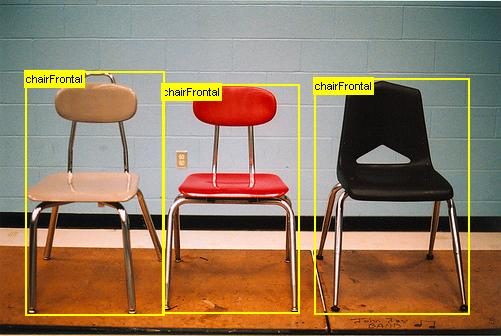
\includegraphics[width=.9\textwidth]{imagem/0x_classdetec.jpg}
% Caption centralizada
  \captionsetup{justification=centering}
  \captionfont{\small{\textbf{\\Fonte: \citeonline{everingham-2015}.}}}	
  \label{fig:exemploclassdet}
  \end{figure}

A Figura \ref{fig:exemploclassdet} mostra exemplos de como devem ser as saídas de um algoritmo de classificação e localização de objetos. Os retângulos destacados em torno dos objetos são resultados do algoritmo de localização que determina que dentro daquela região existe um objeto de interesse e os rótulos destacados em cima dos retângulos são os resultados do algoritmo de classificação, que determina que o objeto contido dentro da região pertence àquela classe.

O uso das \ac{CNN} tem se tornado cada vez mais populares, principalmente em alguns dos problemas clássicos de processamento de imagens. A primeira abordagem desse tipo foi proposta por \citeonline{fukushima-1980} para fazer reconhecimento de caracteres escritos a mão. Mais tarde, \citeonline{lecun-1998} desenvolveram uma arquitetura de \ac{CNN} para a mesma tarefa e obtiveram uma acurácia de $70\%$, sendo essa muito superior aos resultados obtidos por qualquer outro classificador utilizado até então.

%%% p1 Escrever sobre os resultados obtidos pelas CNNs em classificação de imagens
Contudo, as \ac{CNN} só passaram a ser utilizadas com mais frequência algum tempo depois. \citeonline{deng-2009} lançaram o ImageNet, uma base de dados de larga escala com mais de 14 milhões de imagens anotadas manualmente divididas em mais de 22 mil classes diferentes. Essa base de imagens pode ser usada para as tarefas de classificação, detecção e localização de objetos. Além disso, \citeonline{deng-2009} também lançaram o \ac{ILSVRC}, uma competição global anual, aonde os competidores são avaliados nas tarefas de classificação de imagens, detecção de objetos e localização de objetos. \citeonline{krizhevsky-2012} alcançaram o melhor resultado no \ac{ILSVRC} de 2012 usando a AlexNet - uma \ac{CNN} - e desde então, as \ac{CNN}s obtém sempre os melhores resultados nos desafios.

Em \citeyear{he-2016}, \citeauthor{he-2016} propôs a \ac{ResNet} que introduziam o conceito de \textit{skip connection}. Uma \textit{skip connection} é quando a camada $C_n$ além de se conectar com a camada $C_{n+1}$ ela se conecta com outra mais a frente - no caso da \textit{\ac{ResNet}}, a camada $C_{n+2}$. Sendo assim, na entrada $C_{n+2}$ recebe em suas entradas uma junção das saídas de $C_{n}$ e $C_{n+1}$. Essa combinação de entradas na \ac{ResNet} foi feita como uma soma de matrizes. A figura \ref{fig:blocoresidual} mostra um exemplo de \textit{skip connection} na \textit{\ac{ResNet}}.

\begin{figure}[H]
	% Alterar espaçamentos antes e depois do caption
	\setlength{\abovecaptionskip}{0pt}
	\setlength{\belowcaptionskip}{0pt}
	% Caption
	\caption[Exemplo de bloco residual]{Exemplo de bloco residual}
	\centering
	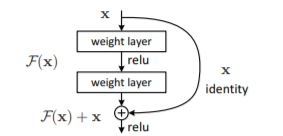
\includegraphics[width=.5\textwidth]{imagem/0x_resnet_arch.jpg}
	% Caption centralizada
	\captionsetup{justification=centering}
	\captionfont{\small{\textbf{\\Fonte: \citeonline{he-2016}.}}}	
	\label{fig:blocoresidual}
\end{figure}

\citeonline{he-2016} alem de vencerem o \ac{ILSVRC} de 2015, venceram o prêmio de melhor artigo na \ac{CVPR} de 2016.

Seguindo a mesma ideia de \textit{skip connection} proposta por \citeonline{he-2016}, \citeonline{liu-2017} propuseram a \ac{DenseNet}. Nessa nova arquitetura houveram duas mudanças com relação à \ac{ResNet}. A primeira mudança é que as saídas das camadas não seriam mais somadas, mas sim concatenadas, ou empilhadas. A segunda é que em um bloco residual as camadas se conectam com todas as suas sucessoras. 

\begin{figure}[H]
	% Alterar espaçamentos antes e depois do caption
	\setlength{\abovecaptionskip}{0pt}
	\setlength{\belowcaptionskip}{0pt}
	% Caption
	\caption[Exemplo de bloco denso]{Exemplo de bloco denso}
	\centering
	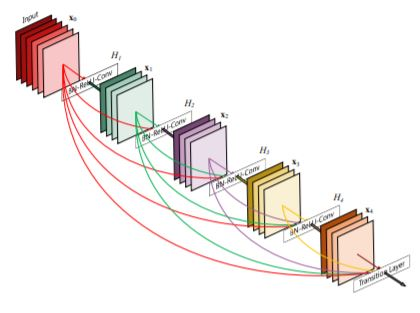
\includegraphics[width=.5\textwidth]{imagem/0x_densenet_block.jpg}
	% Caption centralizada
	\captionsetup{justification=centering}
	\captionfont{\small{\textbf{\\Fonte: \citeonline{liu-2017}.}}}	
	\label{fig:blocodenso}
\end{figure}

A figura \ref{fig:blocodenso} mostra como se conectam as camadas na \ac{DenseNet}. Supondo que temos um bloco denso $B$ com um conjunto de 5 camadas $C = \{c_1, c_2, c_3, c_4, c_5\}$. Como explicado no parágrafo anterior, a saída das camadas serão utilizadas em todas as camadas subsequentes no mesmo bloco. Sendo assim, a entrada de $c_3$ será composta pelas saídas de $c_1$ e $c_2$ concatenadas, e assim sucessivamente. Além disso, como as saídas são concatenadas e não somadas, a tendência é que as entradas cresçam a medida que a rede se aprofunda. O conceito de bloco denso permite propagar múltiplos níveis de abstração ao longo de toda a rede, melhorando assim os resultados obtidos \cite{liu-2017}.

\citeauthor{liu-2017} ficaram em segundo lugar no \ac{ILSVRC} de 2017 e venceram o prêmio de melhor artigo da \ac{CVPR} do mesmo ano.

%%% p2 Escrever sobre os resultados obtidos pelas CNNs em Localização de Objetos
Nas tarefas de localização de objetos as \ac{CNN}s também têm se destacado com bons resultados. \citeonline{redmon-2015} propuseram o \ac{YOLO} e obtiveram um bom resultado fazendo localização e classificação de objetos em tempo real, conseguindo processar 45 \ac{FPS} com uma \ac{mAP} de 63,4\%. \citeonline{sren-2017} propuseram o \ac{R-CNN} e conseguiram obter resultados significativamente melhores para as tarefas de localização e classificação chegando a uma \ac{mAP} de até 78,8\%. Numa implementação alternativa com o enfoque no processamento em tempo real, a \ac{mAP} cai um pouco, chegando a 73,2\% porém, ele processa apenas 7 \ac{FPS}.

\citeonline{wei-2015} propuseram o \ac{SSD}, uma abordagem que além de obter uma \ac{mAP} elevada (74,3\%), supera a velocidade alcançada no \ac{YOLO} atingindo 59 \ac{FPS}. Esses resultados são especialmente relevantes, pois, além de serem competitivos com o estado da arte, trabalham com imagens menores - enquanto os quadros processados pelo \ac{YOLO} têm dimensões $448 \times 448$ e os processados pelo \ac{R-CNN} têm $1000\times 600$, o \ac{SSD} processa quadros de dimensões $300 \times 300$. O principal ganho em trabalhar com imagens menores é diminuir o consumo de memória e ter um método mais robusto por poder obter resultados competitivos mesmo que com imagens menores. Por um outro lado, trabalhar com imagens menores pode significar que o método seja mais lento ao processar imagens maiores.

%%% p3 Escrever sobre os resultados obtidos pelas CNNs em Segmentação semantica usando deconvolução
Uma outra área impactada pelo uso das \ac{CNN}s é a área de segmentação semântica. \citeonline{long-2014} propuseram o uso de uma \ac{FCN} para fazer segmentação semântica e conseguiram obter resultados superiores ao estado da arte, utilizando camadas de deconvolução para aumentar a resolução dos mapas de filtros gerados na saída da \ac{CNN}. \citeonline{noh:2015} propuseram um trabalho mais avançado de forma a tratar algumas limitações encontradas por \citeonline{long-2014}. Essa arquitetura funciona com a estrutura de um \textit{autoencoder}, usando as camadas de deconvolução que não servem para aumentar a resolução, mas para recuperar as informações da imagem de forma mais refinada, de forma a melhorar os resultados da segmentação.

%%% p4 Escrever sobre os resultados obtidos pela DSSD
Por fim, \citeonline{cheng-2017} propôs uma abordagem alternativa na resolução dos problemas de localização e classificação de objetos utilizando camadas de deconvolução a \ac{DSSD}. A \ac{DSSD} recebe essa sigla, pois é uma extensão do \ac{SSD} \cite{wei-2015}. A diferença é que, ao final, ele acrescenta camadas de deconvolução e, com os resultados das deconvoluções ele faz a classificação e a localização. Os resultados obtidos superam os apresentados pelo \ac{SSD} em \ac{mAP}, alcançando 81,5\% embora, o  \ac{DSSD} perde na velocidade (13,6 FPS). 

\section{Motivação}
\label{secao:1:1}

%%% p1 Mencionar como as CNNs tem sido objetos de estudo recentemente
Estudos envolvendo redes neurais convolucionais têm sido realizados com muita frequência tanto em áreas gerais, quanto aplicados à áreas específicas. Estudos vem sendo feitos para classificação de imagens \cite{krizhevsky-2012, simonyan-2014}, classificação e detecção de objetos \citeonline{cheng-2017, lin-2014}, segmentação de imagens \citeonline{long-2014, noh:2015}, segmentação de objetos em vídeos \citeonline{caelles-2017, voigtlaender-2017}. Isso se deve aos bons resultados obtidos pelos métodos aplicados nas respectivas áreas.

%%% p2 Mencionar como as aplicações dos algoritmos de detecção
Além disso, o problema de classificação e detecção de objetos tem sido aproveitado como solução para problemas mais específicos, como detecção facial \cite{yang-2018}, contagem de pessoas \cite{pren-2017} e detecção de pedestres \cite{lan-2018}. 

%%% p3 Mencionar a espectativa ao usar deconvolução
Por fim o uso das camadas de deconvolução no método proposto traz boas expectativas, uma vez que já há resultados na literatura que mostram a sua eficiência \cite{noh:2015, cheng-2017}. Em suma, pode-se dizer que o tema ainda tem muito que ser explorado, que a proposta é promissora, e que bons resultados podem trazer contribuições para trabalhos futuros.

\section{Objetivos}
\label{secao:1:2}  

O objetivo do trabalho é utilizar uma arquitetura de \ac{CNN} modificada com camadas de deconvolução para fazer detecção e classificação de objetos. Para isso, será necessário:

\begin{itemize}
	\item Adaptar a \ac{CNN} \ac{DenseNet} \cite{liu-2017} para fazer localização e classificação de forma similar à \ac{SSD};
	\item Alterar a arquitetura da rede inicial para receber camadas de deconvolução de forma a melhorar os resultados da classificação e da Localização;
	\item Avaliar os resultados obtidos comparando-os com a literatura.
\end{itemize}

\section{Justificativa}
\label{secao:1:3}

Com os avanços tecnológicos alcançados ao longo das últimas décadas, a produção de conteúdo multimídia tem crescido consideravelmente e tem sido amplamente explorada pelos mais diversos setores da sociedade. Todos os dias mais de 95 milhões de fotos e vídeos são postadas no Instagram\footnote{https://www.instagram.com}. Esse imenso volume de dados que são produzidos e acessados em multimídia inviabiliza a manipulação deste conteúdo por meio de ação humana; criando assim, a necessidade de automatizar a recuperação e análise de informações relevantes contidas nas mesmas.

Nesse sentido, todos os dias são estudados novos algoritmos e novas técnicas para fazer recuperação de informação multimídia. E uma das formas amplamente utilizadas é a de localização e classificação de objetos em imagens. \citeonline{everingham-2015} definem que o problema de classificação consiste em responder para cada classe de objeto se existe ou não uma ou mais instâncias daquele objeto na imagem e, o problema de localização consiste em dizer onde na imagem estão as instâncias dos objetos reconhecidos pelo classificador.

É válido estabelecer que ``os mecanismos sensitivos dos seres humanos (como visão e audição) sugerem a necessidade de uma arquitetura profunda para extrair a sua estrutura complexa'' \cite{deng-2014}. Porém, de acordo com \citeonline{caelles-2017}, uma grande limitação ao utilizar arquiteturas de \emph{Deep Learning} é a necessidade de treinamento com um grande volume de dados. Essa limitação torna o processo mais custoso em termos de tempo de processamento e outros recursos computacionais(como memória). Além disso, a base de dados deve ter os resultados da classificação e localização esperados feitos de forma manual, o que aumenta o esforço humano.

Tendo isso em vista, a proposta de utilizar a \ac{DenseNet} \cite{liu-2017} pré-treinada em classificação de imagens visa diminuir o custo por meio do \textit{Transfer Learning}. Além disso, utilizando as camadas adicionais de deconvolução como proposto por \citeonline{cheng-2017}, espera-se obter resultados ainda melhores. Esses resultados melhores repercutiriam de forma positiva em outras áreas relacionadas à localização e classificação de objetos. 

\section{Organização do texto}
\label{secao:1:4}

O Capítulo \ref{cap:2} traz os principais conceitos relacionados à \textit{Deep Learning}, redes neurais artificiais, classificação de objetos em imagens e detecção de objetos em imagens, necessários à compreensão do trabalho. O Capítulo \ref{cap:3} contém um resumo dos trabalhos relacionados à monografia. O Capítulo \ref{cap:4} contém a metodologia a ser seguida para o desenvolvimento do trabalho. Além disso contém um cronograma a ser seguido e a definição das métricas a ser utilizadas para avaliar os resultados obtidos. O Capítulo \ref{cap:5} descreve os experimentos realizados e os resultados obtidos.